
% This template has been edited from the IEEE template available at:
% https://www.ieee.org/conferences/publishing/templates.html
%
% For further help, you may wish to see:#
% https://www.overleaf.com/learn/latex/tables
% https://www.overleaf.com/learn/latex/Inserting_Images
% https://www.overleaf.com/blog/532-creating-and-managing-bibliographies-with-bibtex-on-overleaf

\documentclass[conference]{IEEEtran}
%\IEEEoverridecommandlockouts
% The preceding line is only needed to identify funding in the first footnote. If that is unneeded, please comment it out.
\usepackage{cite}
\usepackage{amsmath,amssymb,amsfonts}
\usepackage{algorithmic}
\usepackage{graphicx}
\usepackage{textcomp}
\usepackage{xcolor}
\usepackage{subfigure}
\usepackage{parskip}
\def\BibTeX{{\rm B\kern-.05em{\sc i\kern-.025em b}\kern-.08em
    T\kern-.1667em\lower.7ex\hbox{E}\kern-.125emX}}
\begin{document}

\title{Comparing Two Different Complete Coverage Path Planning Algorithms Using The E-puck In Webots}

\author{
    \IEEEauthorblockN{Daoming Chen}
    \textit{Department of Mechanical Engineering}\\
    \textit{University of Bristol,UK}
    \IEEEauthorblockN{ta21463@bristol.ac.uk}
    \and
    \IEEEauthorblockN{Yifan Wang}
    \textit{Department of Mechanical Engineering}\\
    \textit{University of Bristol,UK}
    \IEEEauthorblockN{rj21561@bristol.ac.uk}
}

\maketitle

\begin{abstract}
1
\end{abstract}


\section{Introduction}
With the development of mobile robotics and the continuous innovation of robot vacuum cleaner products, path planning algorithms have become particularly important. Path planning algorithms aim to find an optimal path for a mobile robot, which at the same time satisfies that the path always does not intersect any obstacle from the starting point to the ending point in a given environment. The path trajectory generated by the robot path planning plays a navigational role in its movement and guides the robot from the current point to the target point avoiding obstacles. Complete coverage path planning(CPP) is the process of determining the feasible or optimal path trajectory by delineating the boundaries of obstacle and free areas and ensuring that all points in a given environment are visited at least once, given that all spatial maps information is known. CPP algorithm is widely used in robot vacuum cleaners\cite{colegrave1994case}.\\
The boustrophedon cell decomposition (BCD)\cite{lavalle2006planning} and the Backtracking Spiral Algorithm (BSA)\cite{gonzalez2005bsa} are two CPP methods. These two methods are the main methods used by robot vacuum cleaners. One of the reasons why the time to complete a task varies from one robot vacuum cleaner to another is the different choices of CPP algorithms. This work looks to compare the completion times of mobile robots returning to the starting point from the starting point using these two CPP algorithms in different environments to obtain a more efficient algorithm.

\section{Hypothesis Statement}
In the BCD algorithm, boustrophedon\cite{choset1998coverage} means the way ox walks which is the parallel line-covered areas. So the method traverses the entire map environment in parallel lines(see Fig.\ref{bcd}). While the BSA algorithm\cite{Gonzlez2003BSAAC} is filling rectangular regions using a spiral pattern(see Fig.\ref{bsa}).\\
There is a clear difference between the two algorithms. The BCD algorithm has a tighter overall path because of its 180° turns, which are closer together after each turn, In the BSA algorithm,  because of its 90° turns after encountering an obstacle, which is not close together after the turn.BSA algorithm is an outward-to-inward spiral path planning method, and its external route will create a certain distance from the internal route. Its route continuity caused by turning when random obstacles appear in the environment will be relatively poor compared to the BCD algorithm.
Based on these observations, a hypothesis has been developed stating:
\begin{quote}
     In the simple map environment, the efficiency of traversing the entire map is similar for both algorithms because the overall path continuity is similar. However, in complex maps (containing random obstacles), compared to BCD, the dispersion of the BSA path area causes BCD to be more efficient than BSA.
\end{quote}

\begin{figure}[htbp]
\centering
\begin{minipage}[t]{0.48\textwidth}
\centering
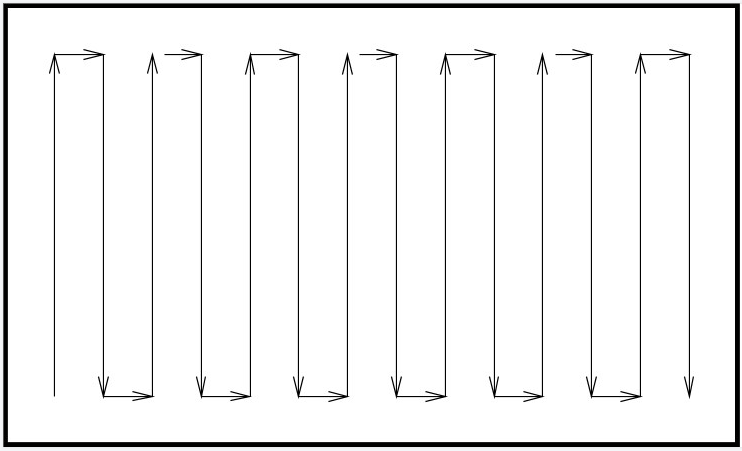
\includegraphics[width=6cm,height=4cm]{RS_Report/bcd.png}
\caption{Diagram of the BCD algorithm\cite{choset1998coverage}. }
\label{bcd}
\end{minipage}
\begin{minipage}[t]{0.48\textwidth}
\centering
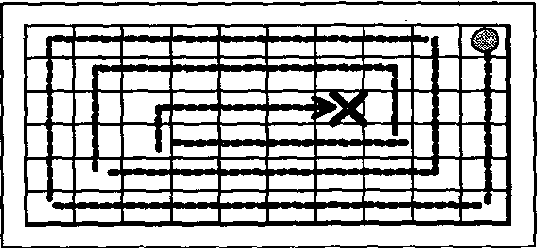
\includegraphics[width=6cm,height=4cm]{RS_Report/BSA.png}
\caption{Diagram of the BSA algorithm\cite{Gonzlez2003BSAAC}.}
\label{bsa}
\end{minipage}
\end{figure}

\section{Implementation}
The individual functions and algorithms required during the experiments were tested separately and a map environment (with obstacles) was developed for the experiments.
\subsection{Map}
In this experiment, the path planning for the E-punk mobile robot starts with obtaining environmental information and establishing an environmental map. A reasonable representation of the environment facilitates the selection of a suitable search algorithm and ultimately achieves a good path with less time overhead. There are various methods to build the environment map, and this experiment mainly uses the raster method\cite{moravec1985high} to build the environment map in a static environment.This method is used because it decomposes the environmental space into local cells and describes the state of the environment in terms of whether obstacles occupy them or not. The maps produced by this method provide accurate metric information and are easier to understand and process than other methods.\\
A 90mm$\times$90mm map(see Fig.\ref{fig1}) was designed in Webots, which contained the obstacles. Since the CPP algorithm for the final comparison was built on a known map environment, in order to be able to tell the E-punk robot about this map, the built map was converted into a static  11$\times$11 raster map(see Fig.\ref{fig2}), where the value of the area within the array corresponding to the area where the map boundary and the obstacle are located was set to 1 and the value of the remaining freely movable area was set to 0.

\begin{figure}[htbp]
\centerline{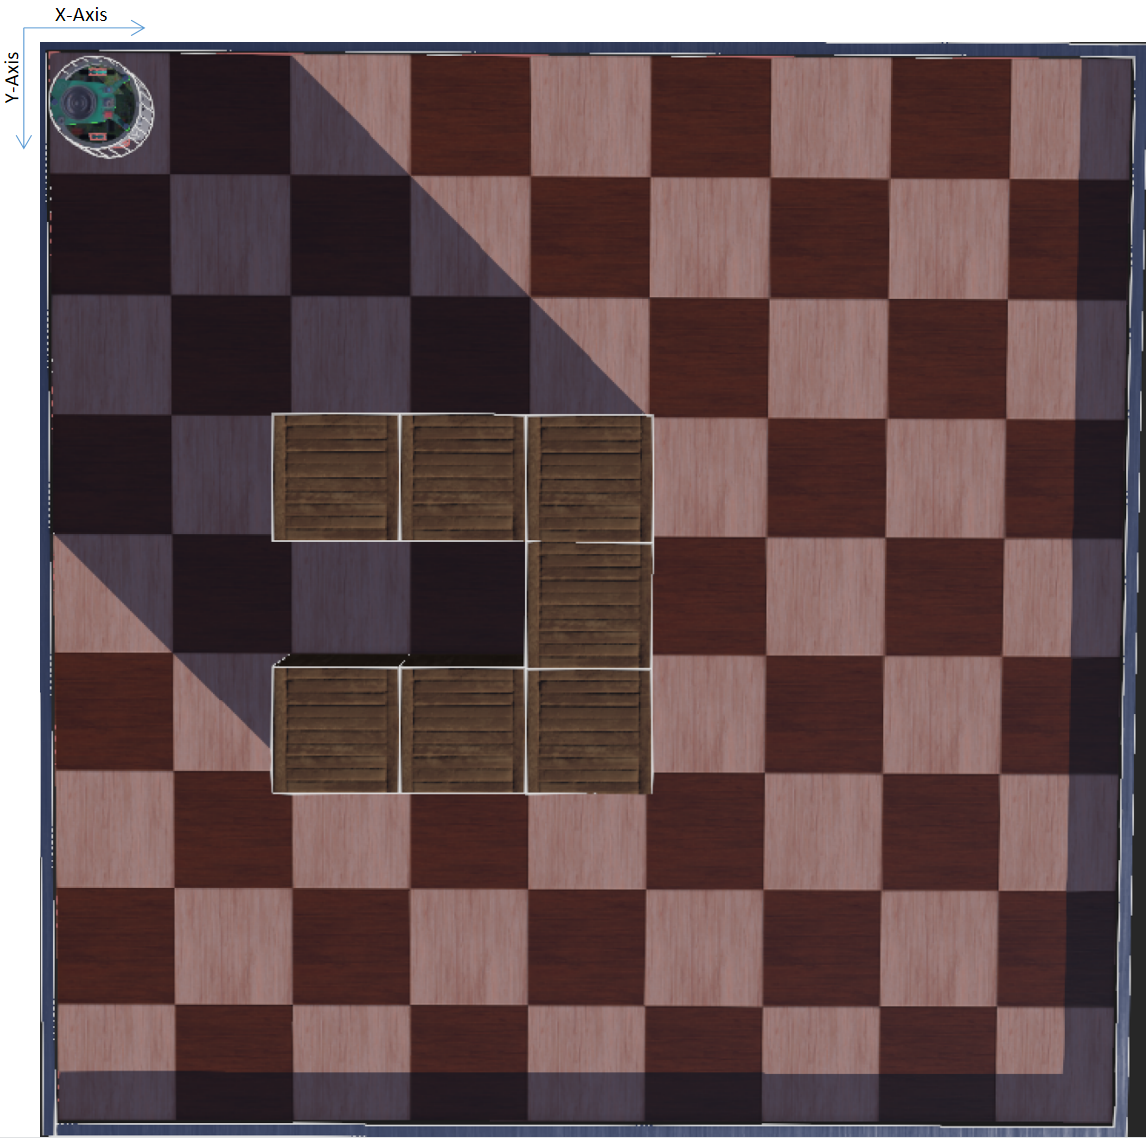
\includegraphics[scale=0.22]{RS_Report/Webots_map.png}}
\caption{E-punk campaign map built in Webots.}
\label{fig1}
\end{figure}

\begin{figure}[htbp]
\centerline{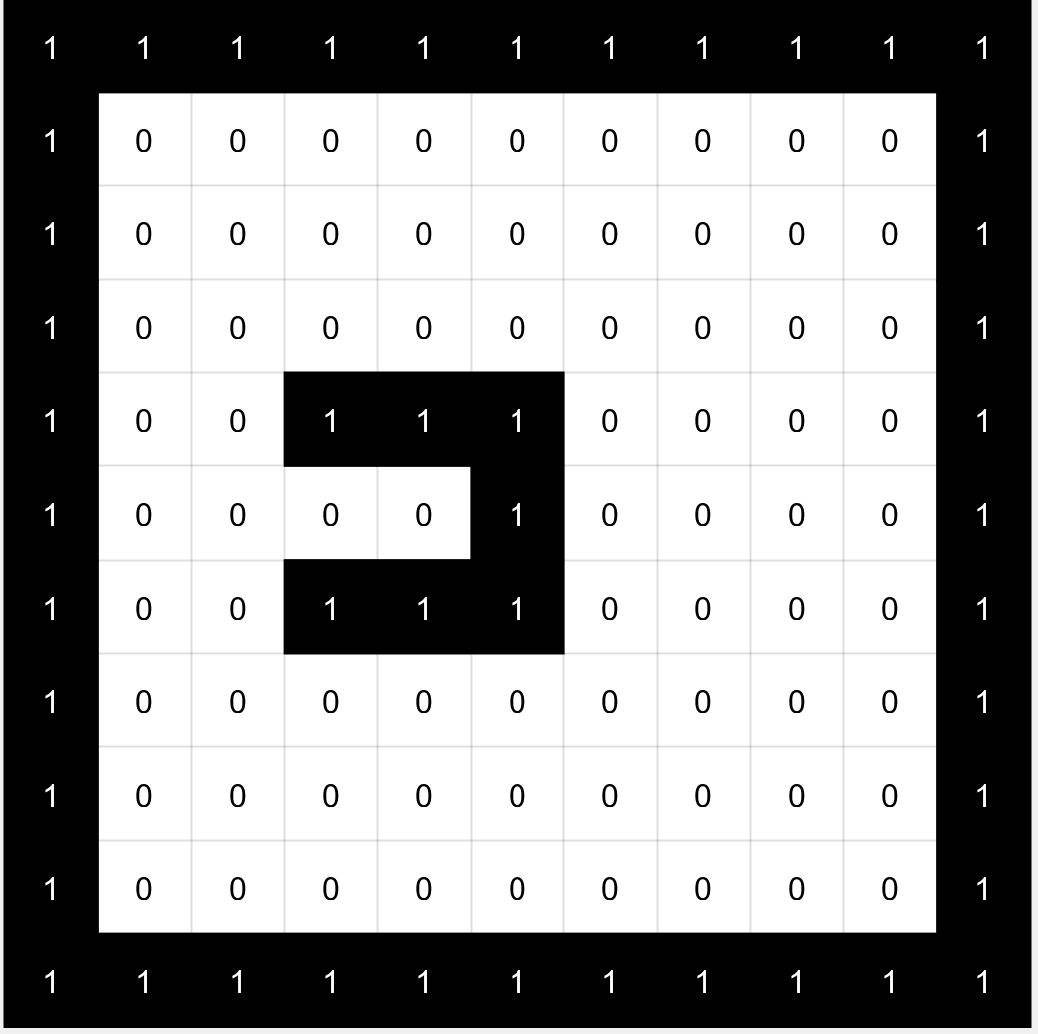
\includegraphics[scale=0.7]{map.png}}
\caption{Raster environment map built for E-punk.}
\label{fig2}
\end{figure}

\subsection{E-punk position}

1\\
1\\
1\\
1\\
1\\
1\\
1\\
1\\
1\\
1\\
1\\
1

\subsection{CPP algorithm}
 Fig.\ref{fig4} shows the overall form of the algorithm architecture combining the map, A* algorithm and CPP algorithm. The architecture allows E-punk to complete the map traversal and compare the completion times of the two different CPP algorithms.
 
\subsubsection{A* algorithm}
The sweeper robot returns to the initial point to recharge after completing the cleaning task in the real world. In this experiment, the robot is set to return to its initial position after completing the CPP task, which is designed to simulate the realistic motion of the robot better. The A* algorithm\cite{hart1968formal} is used to return to the initial position more quickly and with the shortest path.\\

\begin{figure}[htbp]
\centerline{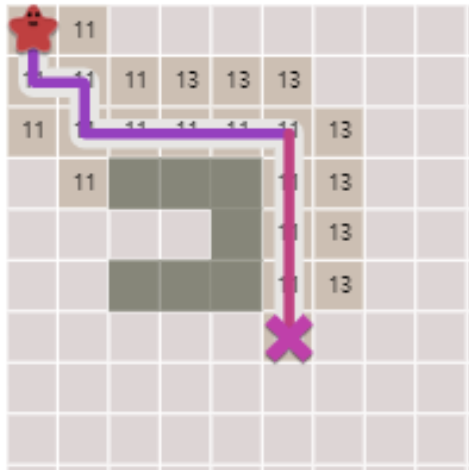
\includegraphics[scale=0.45]{RS_Report/astar.png}}
\caption{A* algorithm demonstration(the value in the cell is the value of $f(n)$).}
\label{fig3}
\end{figure}

As E-punk traverses the map, there will always be places that it has not traversed in a single loop. In this case, the experiment uses the A* algorithm to move the cart to the nearest untraversed region until the entire map is traversed.\\
The core of the a* algorithm is
\begin{equation}
    f(n) = g(n) + h(n)
\end{equation}
where $f(n)$ is the combined priority of node n. When the next node to be traversed needs to be selected, the algorithm always picks the node with the highest combined priority (smallest value). $g(n)$ is the cost of node n from the starting point. $h(n)$ is the expected cost of node n from the end point, which is the heuristic function of the A* algorithm.\\
The traversal direction is simplified in this experiment to match the raster map and speed up the calculation. The mobile robot can only move in four directions, up, down, left and right, in which case the heuristic function is calculated using the Manhattan distance method(see Fig.\ref{fig3}).

\subsubsection{BCD algorithm}
1\\
1\\
1\\
1\\
1\\
1\\
1\\
1\\
1\\

\subsubsection{BSA algprithm}
1\\
1\\
1\\
1\\
1\\
1\\
1\\
1\\
1\\
1
\begin{figure}[htbp]
\centerline{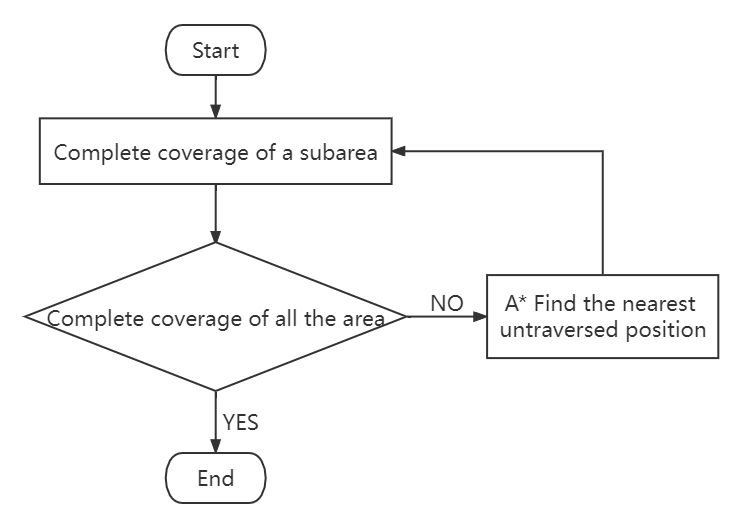
\includegraphics[scale=0.35]{RS_Report/RS_Report.png}}
\caption{Overall architecture of the CPP algorithm.}
\label{fig4}
\end{figure}


\section{Experiment Methodology}

\subsection{Overview of Method}
This experiment compared the completion times of two path planning algorithms, BCD and BSA, on the same map. Because the maps selected for the experiment were raster maps, all maps used for this experiment defined a cell size of 10mm$\times$10mm, and this area was scattered across the raster map. The experiment first verified whether the number of turns would directly affect the completion time. In this validation experiment, a 60mm$\times$100mm map was created. This map was blank and was obstacle-free. By changing the orientation of the E-punk in the initial state, its turn position and number of turns during the map traversal became different. Compare the processing times of the two algorithms in these two different cases and complete this verification.\\
After concluding the validation experiment, the task completion times of the two path planning algorithms mentioned above were compared in different environments. The overall layout of the room on the floor for the robot vacuum cleaner does not usually change significantly except for the movement of people, so in this experiment, all maps are static maps, and obstacles do not move. This section is the central part of the experiment. A 90mm$\times$90mm map was defined, and 10mm$\times$10mm square obstacles were placed at random locations on the map. After the map was constructed, the performance of the two path planning algorithms was compared. After comparing on this map environment, the experiment was carried out in two other, different map environments. This approach aims to reduce the impact of random errors in path planning caused by the particular location of some map obstacles. Because the Webots simulation software came with a time counter, the completion time was output when the simulation of both path algorithms ended. Webots is a simulator where the experiment does not require multiple experiments in a single environment to reduce random errors. During the E-punk's movement, the coordinates of the locations it travelled were recorded in real-time, and the set of path coordinates, which was used to visualise the route, was exported when the task was completed.
\subsection{Discussion of Variables}
In this experiment, it is necessary to control that the initial conditions are the same for both algorithms when comparing on the different maps. The starting position of the E-punk is the same for both algorithms. The experiments all started at the global coordinate system $(x, y, \theta) = (0, 0, 0)$, which in the simulated map was located in the top left corner of the map (see Fig.\ref{fig1}). The E-punk's straight ahead speed and turning speed are constant for both path planning algorithms, and these two values do not change from one map to another. The heuristic function used in the A* algorithm is based on the Manhattan distance, which does not change during the comparison. The motion parameters in this algorithm are also unchanged.

\subsection{Discussion of Metric(s)}
In this experiment, the metrics obtained were collected to evaluate the two path planning algorithms' efficiency and compare them. As proposed in the hypothesis, these metrics were chosen to get the efficiency of the two algorithms and the main effects that lead to their difference. Table 1 details the metrics chosen for this experiment.

\begin{table}[htbp]
\centering
\caption{Definition of metrics and their sources}
\label{Table1}
\begin{tabular}{c|l|c}
\hline
Metric                               & \multicolumn{1}{c|}{Source of Metric} & Justification          \\ \hline
Time(s)                              & Internal timer                        & Length of mapping time \\ \hline
\end{tabular}
\end{table}

Both metrics in this experiment can be obtained directly from the timer within Webots and the counter. In this experiment, as a measure of efficiency, it is better to measure time rather than distance travelled, as distance travelled does not consider the time taken to make a turn very well. Also, this experiment compares efficiency with the number of turns made during the path planning process, so this experiment is better suited to using completion time as a measure.


\section{Results}


\section{Discussion and Conclusion}

Begin your discussion and conclusion by re-stating your hypothesis.  You can literally copy-and-paste your hypothesis here.  

Because the VL1680X has been identified as an active sensor with ... limitations, we hypothesised that:
\begin{quote}
    by applying ... filtering to the sensor, we predict a measurable improvement of the sensor under ... conditions.  
\end{quote}


\bibliographystyle{ieeetr} 
\bibliography{biblio}


\end{document}
